\section{Aufbau und Durchführung}
\label{sec:aufbauUndDurchfuehrung}

Im Versuch wird der in Abbildung \ref{fig:aufbau} dargestellte Versuchsaufbau verwendet.
Die verwendeten Halbleiter sind für infrarotes Licht durchlässig, sodass das Experiment
darauf ausgerichtet werden muss. Daher werden als Lichtquelle Halogenlampen verwendet,
deren Spektrum zu großen Teilen aus Infrarotlicht besteht.

\begin{figure}
  \centering
  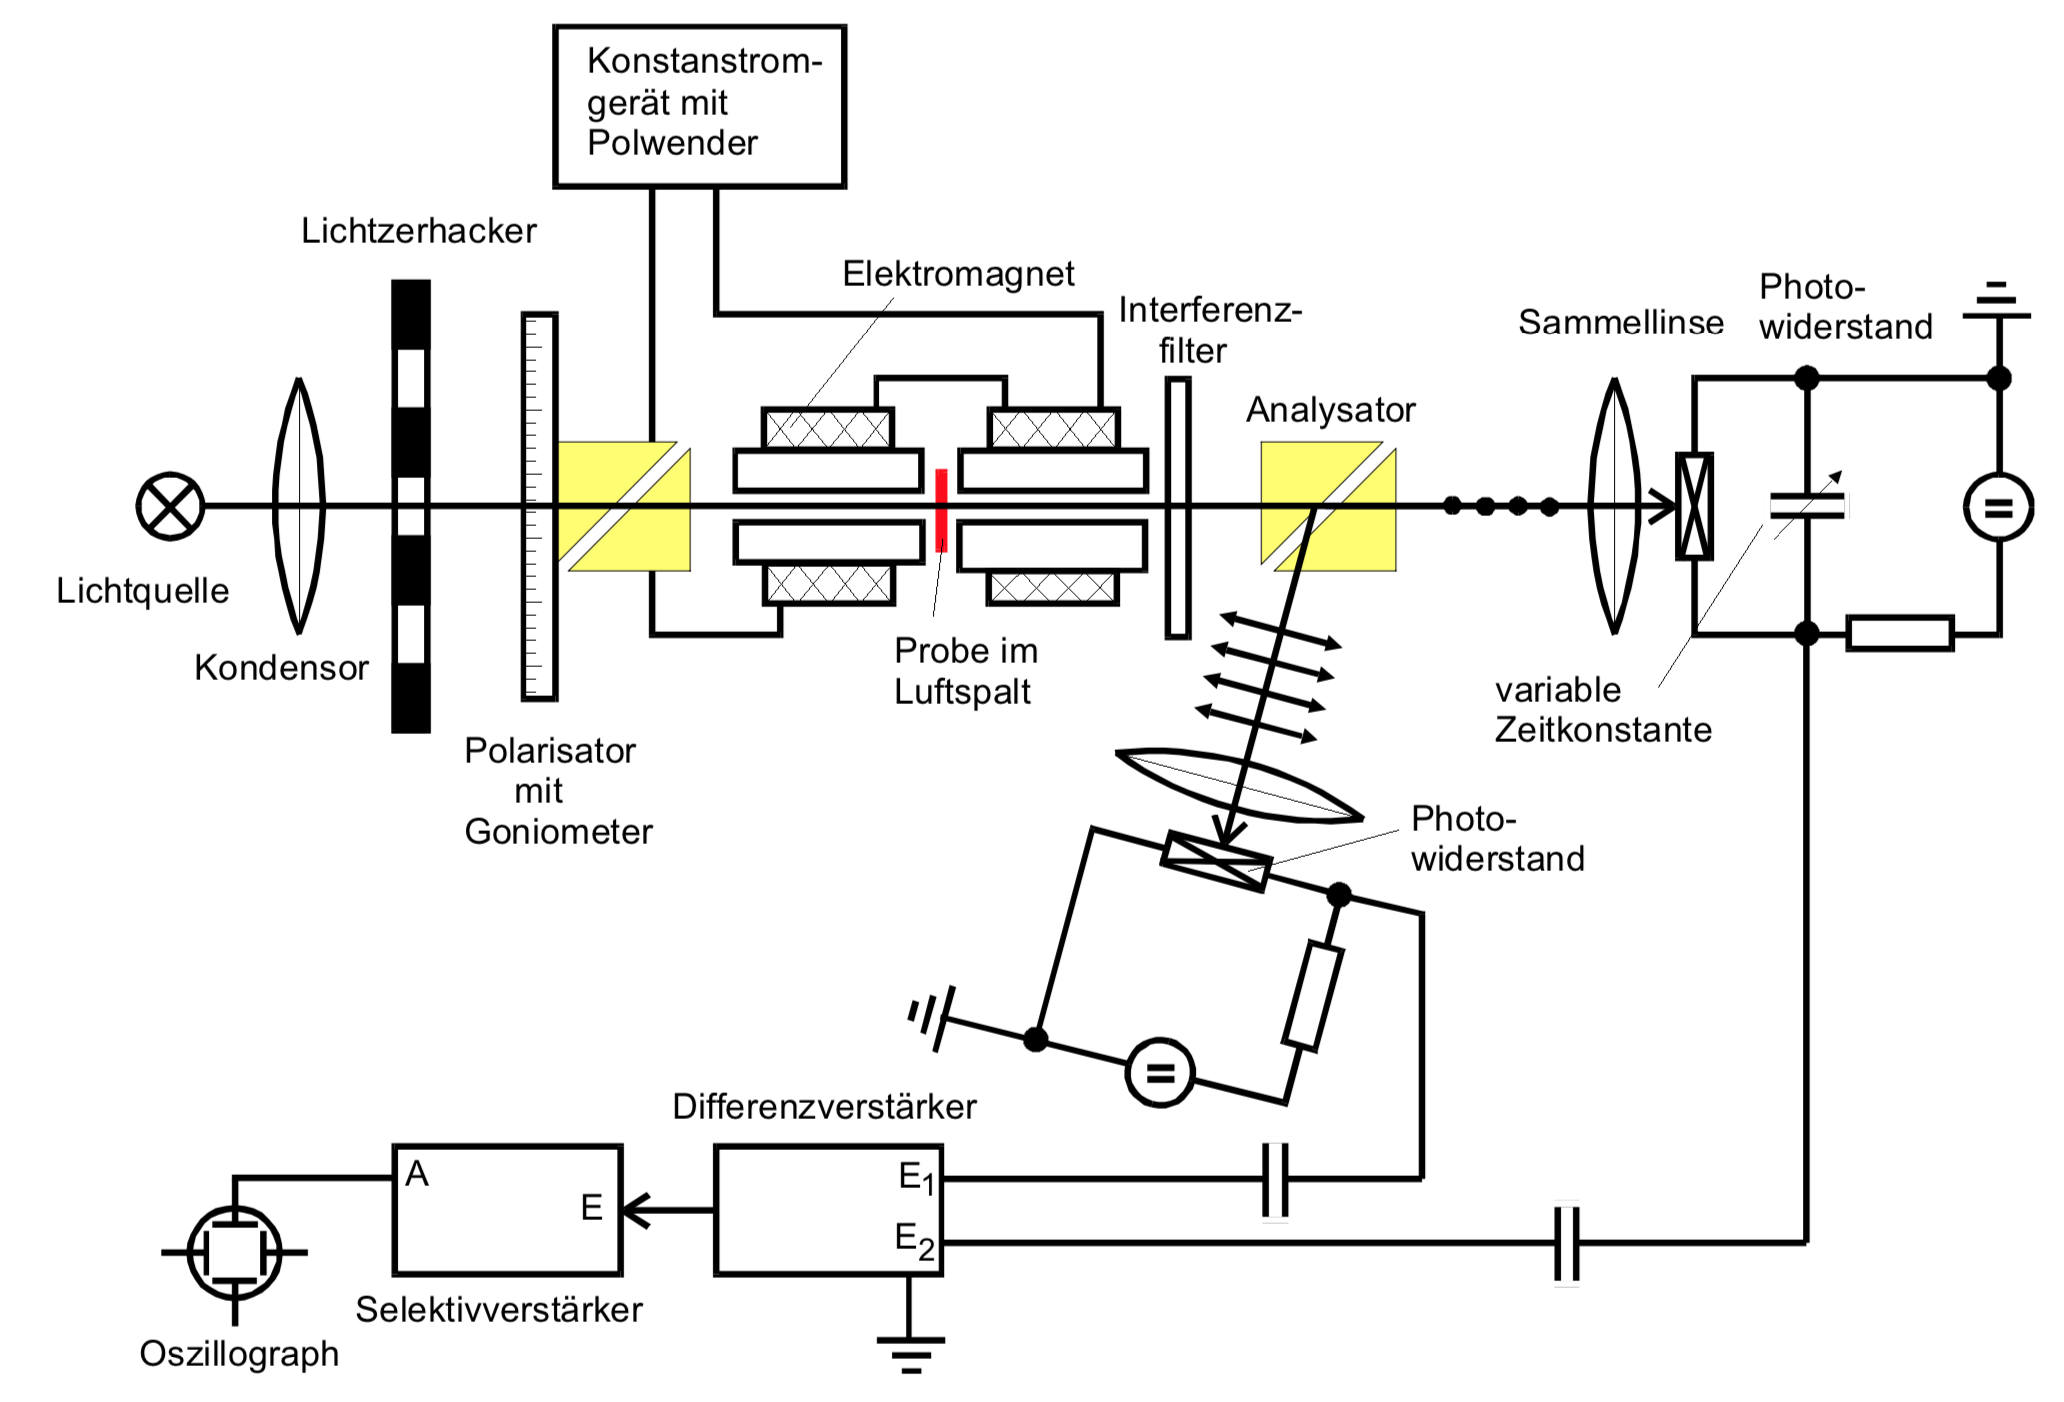
\includegraphics[width=\textwidth]{data/aufbau.png}
  \caption{Schematische Darstellung des Versuchsaufbaus. \cite{anleitung}}
  \label{fig:aufbau}
\end{figure}

Nachdem das Licht durch eine Kondensorlinse gebündelt wurde, fällt es auf einen
sog. Lichtzerhacker. Dies ist ein rotierendes Rad, das das zuvor zeitlich kontinuierlich
vorliegende Licht in kurze Lichtpulse zerhackt. Danach fällt es auf einen Polarisator.
In diesem Versuch wird dafür ein Glan-Thompson-Prisma verwendet. Dieses besteht aus
zwei rechtwinkligen Prismen aus doppelbrechendem Material, die aufeinander geklebt sind.
Das ist auch in Abbildung \ref{fig:gt} zu sehen. Trifft ein zunächst unpolarisierter
Lichtstrahl auf das Prisma, so werden seine s- und p-polarisierten Komponenten wegen der
unterschiedlichen Brechungsindices unterschiedlich an der Grenzfläche reflektiert.
Dabei wird die s-polarisierte Komponente an der Grenzfläche totalreflektiert und die
p-polarisierte Komponente transmittiert, sodass sich der Strahl in einen ordentlichen (s-polarisiert)
und einen außerordentlichen (p-polarisiert) Strahl aufteilt.

\begin{figure}
  \centering
  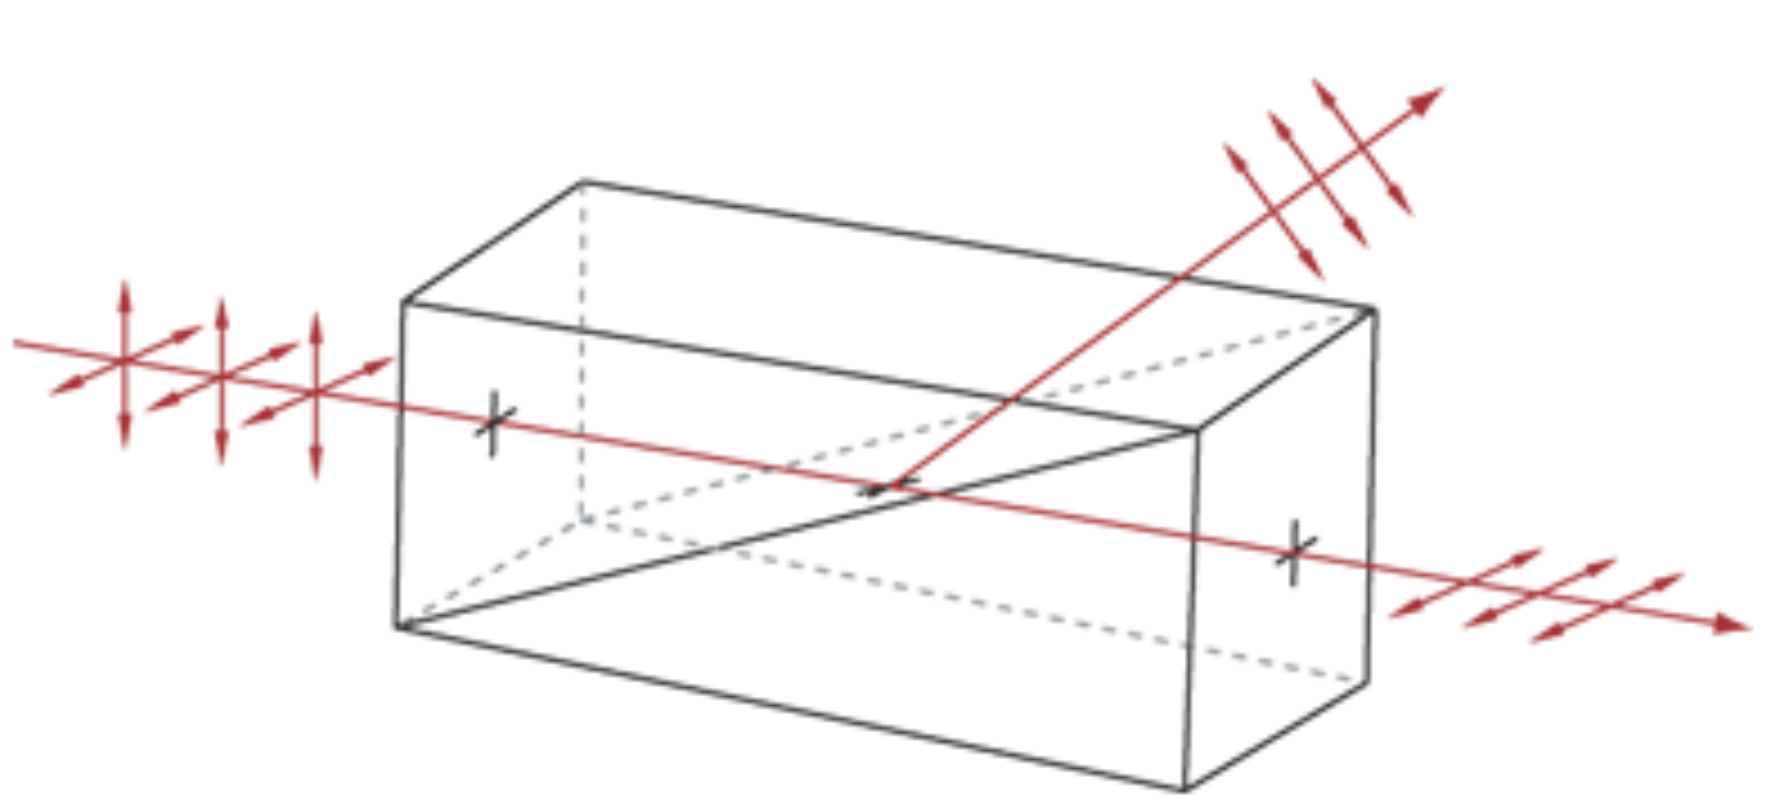
\includegraphics[width=0.6\textwidth]{data/glanthompson.png}
  \caption{Skizze der Funktionsweise eine Glan-Thompson-Prismas. \cite{gt}}
  \label{fig:gt}
\end{figure}

Durch das Glan-Thompson Prisma wird der zunächst unpolarisierte Strahl linear
polarisiert. Dieser linear polarisierte Strahl trifft dann auf die Probe, die ich
im magnetischen Feld eienes Elektromagneten befindet. Darauf folgt ein Interferenzfilter,
in dem eine bestimmte Lichtfrequenz herausgefiltert wird. Dieser besteht aus einer dünnen
Schicht eines Dielektrikums, das von zwei semitransparenten Schichten umgeben ist.
Das einfallende Licht wird an jeder Grenzfläche teilweise reflektiert und teilweise
transmittiert, sodass viele Teilstrahlen entstehen, die daraufhin miteinander
interferieren können. Konstruktive Interferenz tritt nur dann auf, wenn die spezielle
Interferenzbedinung des Interferenzfilters (abhängig von seiner Dicke und seinem Brechungsindex)
erfüllt wird. Alle anderen Frequenzen löschen sich durch Interferenzen aus. Eine Skizze
zur Funktionsweise des Interferenzfilters befindet sich in Abbildung \ref{fig:if}

\begin{figure}
  \centering
  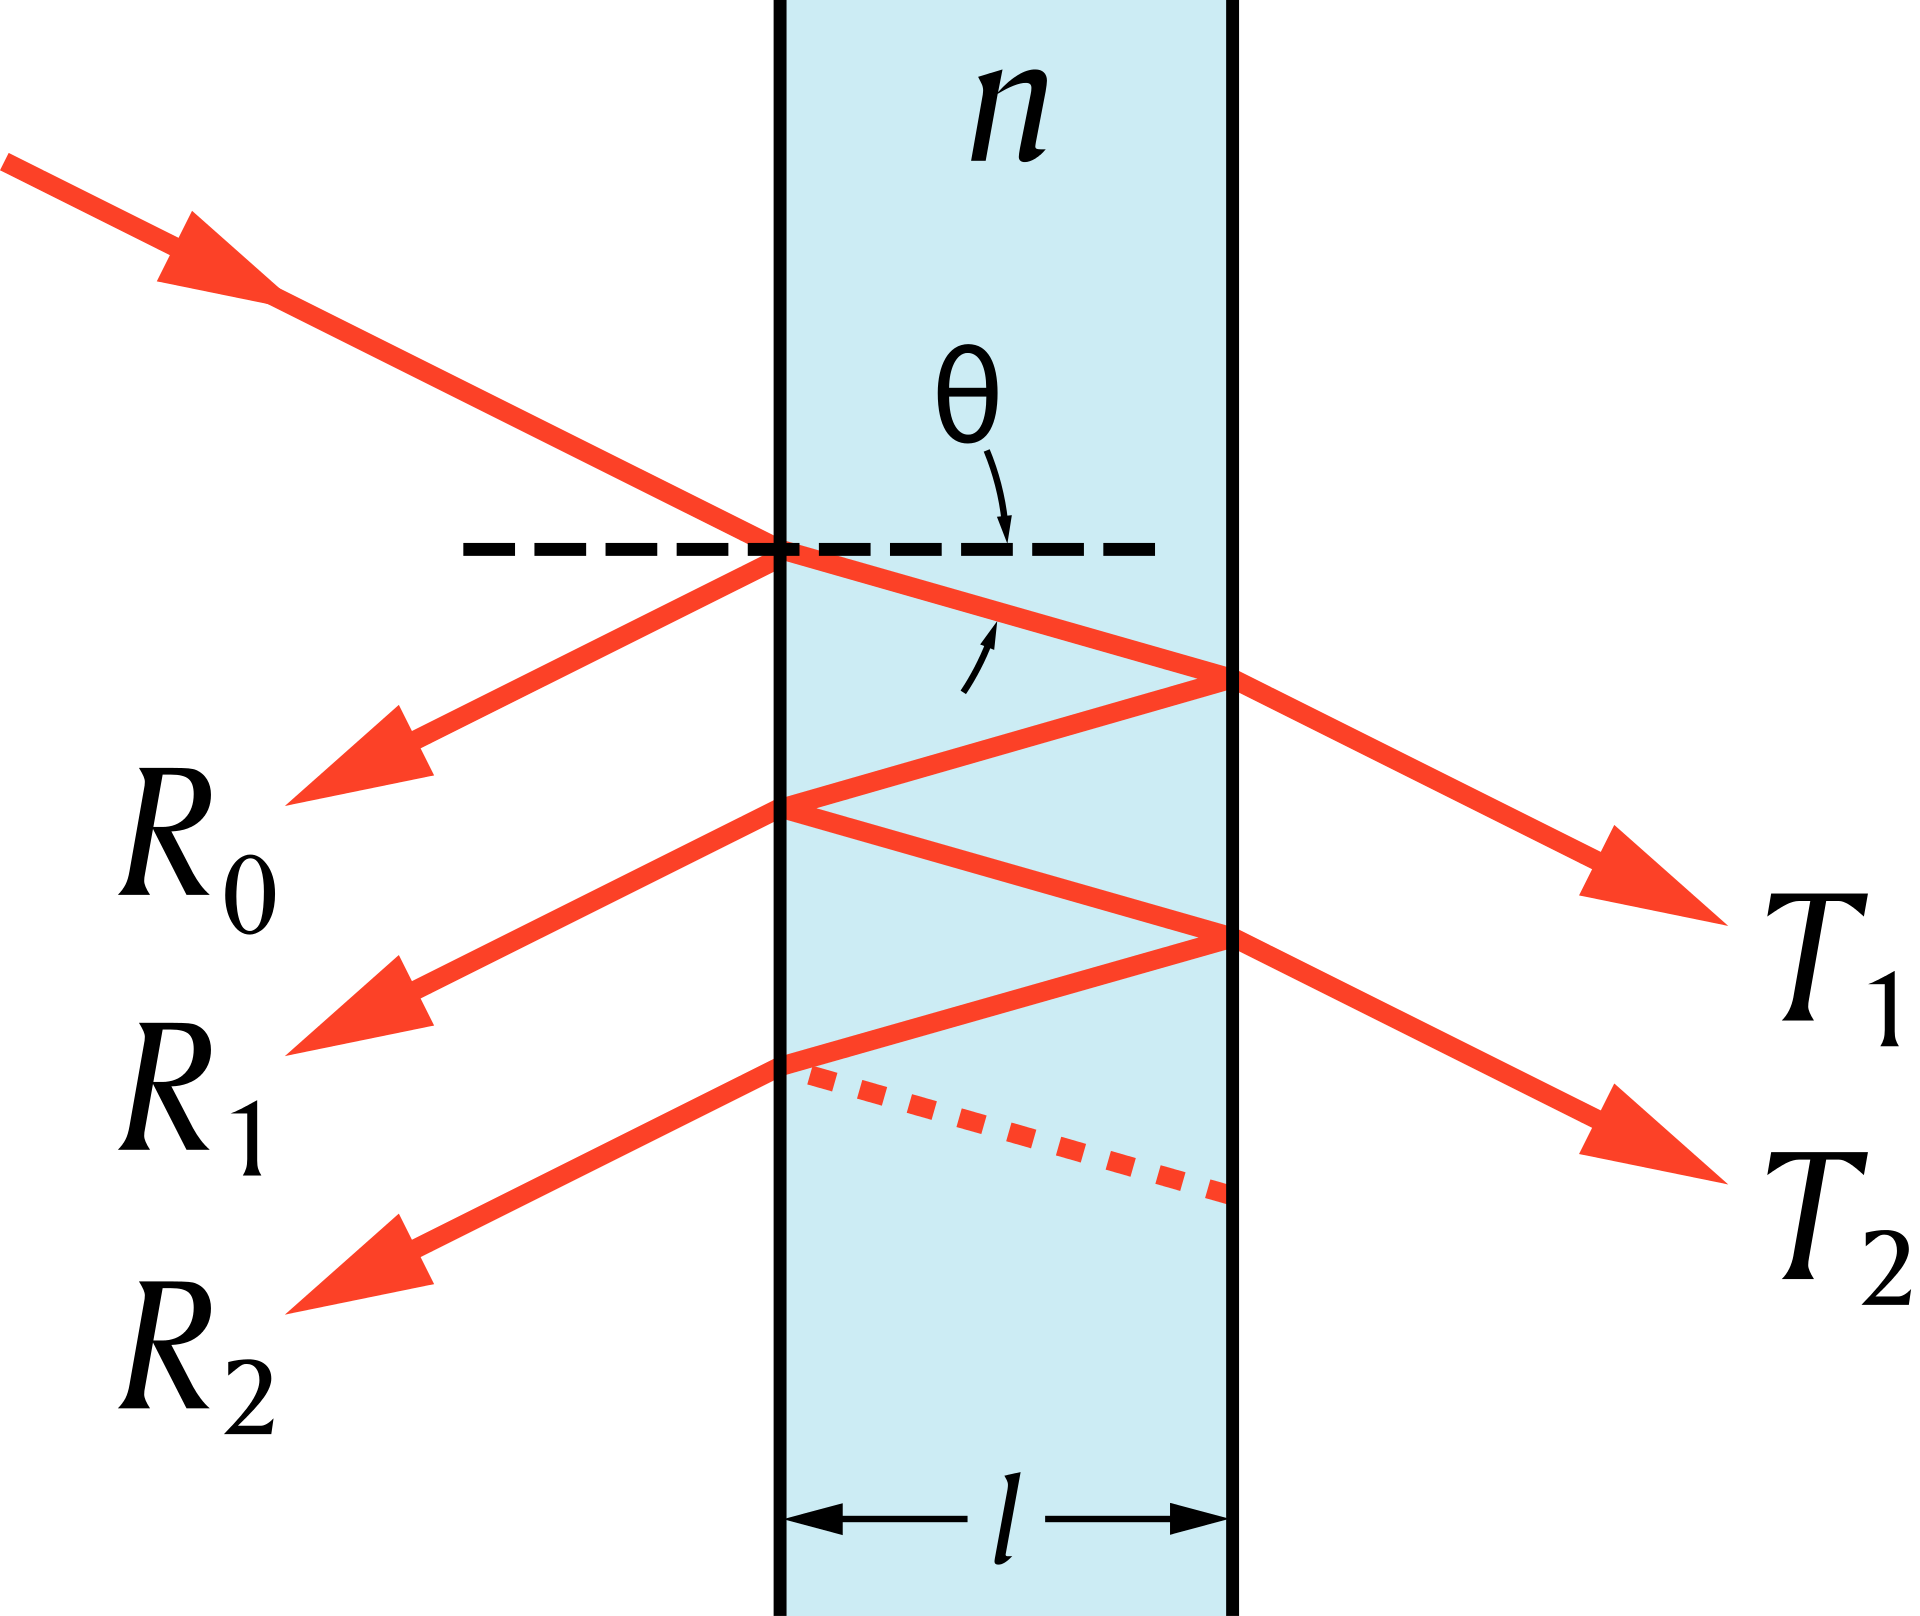
\includegraphics[width=0.5\textwidth]{data/if.png}
  \caption{Skizze der Funktionsweise eines Interferenzfilters. \cite{wiki2}}
  \label{fig:if}
\end{figure}

Das gefilterte Licht trifft auf ein zweites Glan-Thompson-Prisma, das hier als Analysator dient.
Aus dem Prisma treten zwei senkrecht zueinander polarisierte Strahlen aus, die durch zwei
Photowiderstände gemessen werden. Die an den Photowiderständen
gemessenen Spannungen werden auf einen Differenzverstärker gegeben. Die Ausgangsspannung
desselben ist dann proportional zur Differenz der beiden gemessenen Spannungen. Sie
ist genau dann null, wenn beide Wellen identisch sind. Die Frequenz des Differenzverstärkers
wird  mithilfe des Selektivverstärkers auf die des Zerhackers abgestimmt. Die Ausgangsspannung
wird auf ein Oszilloskop gegeben.

Zur Messung des Winkels $\theta$ wird bei maximalem magnetischen Feld Frequenz des Selektivverstärkers
auf die des Zerhackers eingestellt, indem am Oszilloskop ein Maximum der Ausgangsspannung gesucht wird.
Danach wird das erste Glan-Thompson-Prisma
gedreht und die Ausgangsspannung damit auf ein Minimum geregelt. Der entsprechende
Winkel wird notiert. Danach wird das magnetische Feld umgepolt und es wird erneut
durch Drehung des ersten Glan-Thompson-Prismas ein Minimum der Ausgangsspannung gesucht,
dessen Winkel notiert wird. Der Winkel $\theta$ lässt sich dann durch den Zusammenhang
\begin{equation}
  \theta  = \frac{1}{2} (\theta_2 - \theta_1)
\label{eqn:drehwinkel}
\end{equation}
bestimmen. Dabei ist $\theta_1$ der beim in die einer Richtung gepolten Magnetfeld gemessene Winkel und
$\theta_2$ der beim in die andere Richtung gepolten Magnetfeld gemessene Winkel.

Mithilfe der beschriebenen Apparatur und des erklärten Verfahrens werden im Versuch zwei dotierte
und eine hochreine Probe aus Galliumarsenid (GaAs) untersucht. Um später die effektive Masse berechnen zu
können, wird außerdem das magnetische Feld am Ort der Probe mit einer Hall-Sonde gemessen.
